\documentclass[a4paper]{article}

%% Language and font encodings
\usepackage[english]{babel}
\usepackage{amsthm}
\usepackage[utf8x]{inputenc}
\usepackage[T1]{fontenc}
\usepackage{listings}
\usepackage{algpseudocode, algorithm}
\usepackage{mathtools}
\usepackage{enumerate}
\usepackage{tabu}
\usepackage{subfig}

%% Sets page size and margins
\usepackage[a4paper,top=3cm,bottom=2cm,left=3cm,right=3cm,marginparwidth=1.75cm]{geometry}

%% Useful packages
\usepackage{amsmath}
\usepackage{graphicx}
\usepackage[colorinlistoftodos]{todonotes}
\usepackage[colorlinks=true, allcolors=blue]{hyperref}

\newenvironment{solution}{\begin{proof}[\textnormal{\textbf{Solution}}]}{\end{proof}}
\newenvironment{exercise}[1]{\begin{proof}[\textnormal{\textbf{Exercise #1:}}]\phantom{\qedhere}}{\end{proof}}
\newenvironment{lemma}{\begin{proof}[\textnormal{\textbf{Lemma}}]\phantom{\qedhere}}{\end{proof}}
\newenvironment{definition}[1]{\begin{proof}[\textnormal{\textbf{Definition: #1}}]\mbox{}\\\phantom{\qedhere}}{\end{proof}}

\setcounter{secnumdepth}{4}
\setcounter{tocdepth}{4}

\theoremstyle{definition}
\newtheorem*{thm}{Theorem}

\renewcommand\thesubfigure{\arabic{subfigure}}

\begin{document}
\begin{titlepage}\pagenumbering{gobble}
	\centering
	{\scshape\LARGE University of Houston\par}
	\vspace{1cm}
	{\scshape\Large Final-Exam Review \par}
	\vspace{1.5cm}
	{\huge\bfseries COSC 3320 \par}
	{\huge\bfseries Algorithms and Data Structures\par}
	\vspace{0.5cm}
	{\large\bfseries Gopal Pandurangan\par}
	\vspace{2cm}
	\vfill

% Bottom of the page
\end{titlepage}
\vspace*{\fill}\begin{center}{\Huge This page intentionally left blank.}\end{center}\vspace*{\fill}\thispagestyle{empty}\clearpage
\pagenumbering{arabic}
\setcounter{section}{-1}
\section{Previous Concepts}
Concepts seen previously can be found in the mid-term review, located \href{https://github.com/KalHourani/algorithms-and-data-structures-mid-term-review/raw/master/mid-term-review.pdf}{here}.
\setcounter{section}{0}
\section{Greedy Algorithms}
A \textbf{Greedy Algorithm} will make the \textit{locally optimal} choice at each step. A greedy algorithm is not always optimal, but in many cases is optimal or sufficiently close to the optimal solution to justify its use. Consider the \textbf{Unbounded Knapsack Problem}: given $n$ items with weights $w_1,w_2,\hdots, w_n$ and values $v_1,v_2,\hdots, v_n$, and a weight-limit $W$, determine the non-negative integers for each item, $c_i$, such that \begin{align*}\sum_{i=1}^nc_iv_i&\text{ is maximal}\\\sum_{i=1}^nc_iw_i&\leq W\end{align*}

A greedy solution is to choose the ``best'' item at each step. Sort the items by their ratios of value to weight, $\frac{v_i}{w_i}$, and insert the maximum possible number of copies of the first item, then the second, and so on. This algorithm is not optimal: suppose our items, $\{n_1,n_2,n_3\}$ have weights $\{2,3,4\}$ and values $\{4,6,9\}$, with a maximum weight of 5. The algorithm will output $\{n_3\}$, which has a value of 9, when $\{n_2,n_1\}$ has a value of 10.

\section{Graphs}
A graph is a collection of vertices (also called nodes) and edges between them. There are two types of graphs: directed and undirected. In a directed graph, an edge has a direction or orientation. In an undirected graph, edges have no direction. 

A cycle is a collection of vertices in a graph such that a vertex can be reached from itself. In an undirected graph with no cycle, there are at most $n \choose 2=\frac{(n)(n-1)}{2}$. In a directed graph, this is doubled, and is simply $(n)(n-1)$. 
\subsection{Representing a Graph}
A graph can be represented in three ways:
\begin{enumerate}
 \item An \textbf{adjacency list}, in which each vertex stores a list of adjacent vertices.
 \item An \textbf{adjacency matrix}, a matrix $A$ where $A_{i,j}=1$ if and only if there is an edge between the $i^{\text{th}}$ and $j^{\text{th}}$ vertices.
\end{enumerate}

Let $n$ denote the number of vertices and $m$ the number of edges. The space and time complexity of the above representations are given in the following table:
\begin{center}
\begin{tabular}{|c|c|c|}\hline
 & Adjacency List & Adjacency Matrix\\\hline
 Space Complexity & $O(n+m)$ & $O(n^2)$\\\hline
 Add vertex & $O(1)$ & $O(n^2)$\\\hline
 Add edge & $O(1)$ & $O(1)$\\\hline
 Remove vertex & $O(m)$ & $O(n^2)$\\\hline
 Remove edge & $O(n)$ & $O(1)$\\\hline
 Check vertices are adjacent & $O(n)$ & $O(1)$\\\hline
\end{tabular}
\end{center}
\subsection{Depth-First Search}
A \textbf{Depth-First Search} (DFS) is a recursive algorithm for searching every vertex of a graph. Begin with some vertex, $v$, and perform the DFS on its unvisited neighbors. This has the following pseudocode:

\begin{algorithm}[H]
\renewcommand{\thealgorithm}{}
\caption{DFS(G, v): depth-first search of $G$ starting at node $v$}\label{iter-dfs}
\begin{algorithmic}[1]
\Procedure{DFS}{G, v}
\State \textbf{mark} $v$ as visited
\For{all neighbors $u$ of $v$}
  \If{$u$ is not visited}
    \State call \Call{DFS}{$G,u$}
  \EndIf
\EndFor
\EndProcedure
\end{algorithmic}
\end{algorithm}

This algorithm runs in linear, $O(n+m)$ time, where $n$ is the number of vertices and $m$ is the number of edges. It uses $O(n)$ memory to store the stack of vertices in the worst case. 
\subsection{Breadth-First Search}
A \textbf{Breadth-First Search} (BFS) is an iterative algorithm for searching every vertex of a graph. Begin with some vertex, $v$, and visit each of its unvisited neighbors. Repeat on the neighbors of the newly visited vertices, and repeat. This is typically done with a queue. 

\begin{algorithm}[H]
\renewcommand{\thealgorithm}{}
\caption{BFS(G, v): breadth-first search of $G$ starting at node $v$}\label{iter-dfs}
\begin{algorithmic}[1]
\Procedure{BFS}{G, v}
\State $Q$ = queue()\Comment{$Q$ is a queue of which vertices to explore.}
\State \textbf{enqueue} $v$ to $Q$
\While{$Q$ is not empty}
  \State $a=\textbf{dequeue}(Q)$\Comment{Dequeue the queue and visit.}
  \For{neighbors $u$ of $a$}
    \If{$u$ is unvisited}
      \State \textbf{enqueue} $u$ to $Q$
      \State \textbf{mark} $u$ as visited
    \EndIf
  \EndFor
\EndWhile
\EndProcedure
\end{algorithmic}
\end{algorithm}

This algorithm runs in linear, $O(n+m)$ time, where $n$ is the number of vertices and $m$ is the number of edges. It uses $O(n)$ memory to store the stack of vertices in the worst case. 
\section{Graph Algorithms}
\subsection{Minimum Spanning Tree}
A \textbf{Minimum Spanning Tree} (MST) is a subset of the edges of a connected, edge-weighted undirected graph that connects all vertices and minimizes the total weight. In a case where the edge-weights are unique, the MST will be unique as well. A simple induction proof shows that the MST on a connected graph with $n$ vertices will have $n-1$ edges. 

We present three algorithms to determine the MST and perform each on the following graph:

\begin{center}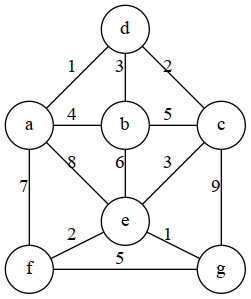
\includegraphics[scale=0.5]{graphs/minimum-spanning-trees/e_1.png}\end{center}

\subsubsection{Kruskal's Algorithm}
Begin with an empty tree. Sort the edges by weight and add the smallest remaining edge to tree \textit{if it does not create a cycle}. Repeat until you have $n-1$ edges in your tree. 
\setcounter{subfigure}{0}

\begin{figure}[H]\centering
 \subfloat[]{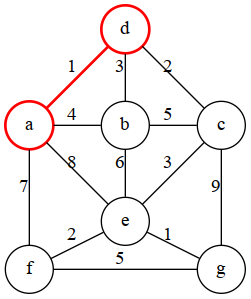
\includegraphics[width=0.33\textwidth]{graphs/minimum-spanning-trees/e_1_k_1.png}}~
 \subfloat[]{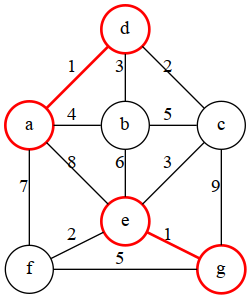
\includegraphics[width=0.33\textwidth]{graphs/minimum-spanning-trees/e_1_k_2.png}}~
 \subfloat[]{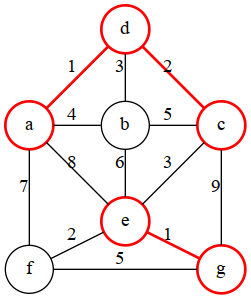
\includegraphics[width=0.33\textwidth]{graphs/minimum-spanning-trees/e_1_k_3.png}}

 \subfloat[]{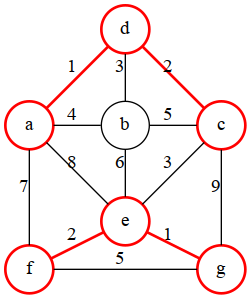
\includegraphics[width=0.33\textwidth]{graphs/minimum-spanning-trees/e_1_k_4.png}}~
 \subfloat[]{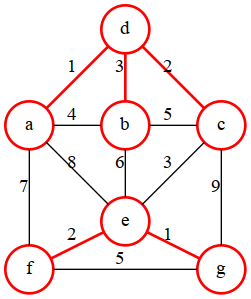
\includegraphics[width=0.33\textwidth]{graphs/minimum-spanning-trees/e_1_k_5.png}}~
 \subfloat[]{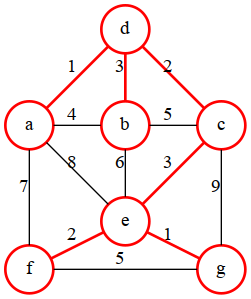
\includegraphics[width=0.33\textwidth]{graphs/minimum-spanning-trees/e_1_k_6.png}}
 \end{figure}
 \begin{figure}[H]\centering
 \subfloat[]{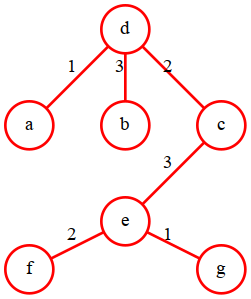
\includegraphics[width=0.33\textwidth]{graphs/minimum-spanning-trees/e_1_k_7.png}}
\end{figure}
\subsubsection{Prim's Algorithm}
Begin with an empty tree. Start at any vertex of the graph. At each step, append the smallest edge that connects the vertices in the MST to the vertices not yet in the MST. Repeat until all vertices are in the tree.
\setcounter{subfigure}{0}

\begin{figure}[H]\centering
 \subfloat[]{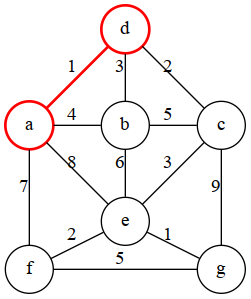
\includegraphics[width=0.33\textwidth]{graphs/minimum-spanning-trees/e_1_p_1.png}}~
 \subfloat[]{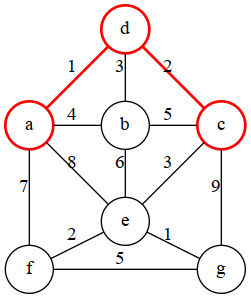
\includegraphics[width=0.33\textwidth]{graphs/minimum-spanning-trees/e_1_p_2.png}}~
 \subfloat[]{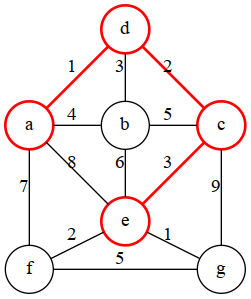
\includegraphics[width=0.33\textwidth]{graphs/minimum-spanning-trees/e_1_p_3.png}}

 \subfloat[]{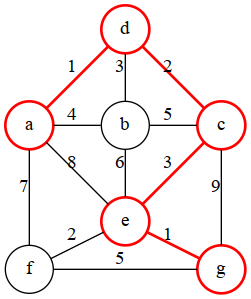
\includegraphics[width=0.33\textwidth]{graphs/minimum-spanning-trees/e_1_p_4.png}}~
 \subfloat[]{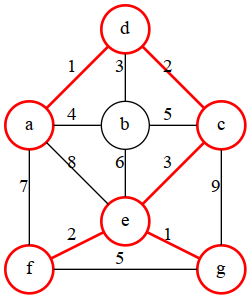
\includegraphics[width=0.33\textwidth]{graphs/minimum-spanning-trees/e_1_p_5.png}}~
 \subfloat[]{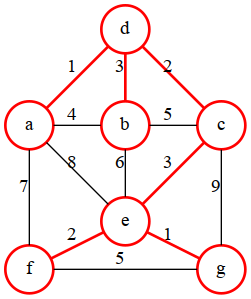
\includegraphics[width=0.33\textwidth]{graphs/minimum-spanning-trees/e_1_p_6.png}}
 \end{figure}
\begin{figure}[H]\centering
 \subfloat[]{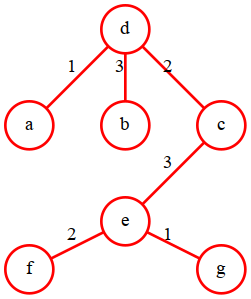
\includegraphics[width=0.33\textwidth]{graphs/minimum-spanning-trees/e_1_p_7.png}}
\end{figure}

\subsubsection{Boruvka’s algorithm}
Begin with an empty tree and with all vertices of the graph as separate components. At each step, add the smallest edge connected to each component to the tree (these edges will not necessarily be unique). Repeat until all vertices are in the tree. 
\setcounter{subfigure}{0}

\begin{figure}[H]\centering
 \subfloat[]{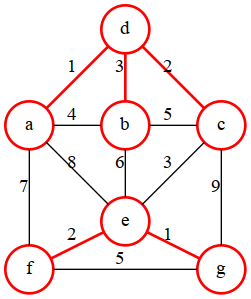
\includegraphics[width=0.33\textwidth]{graphs/minimum-spanning-trees/e_1_b_1.png}}~
 \subfloat[]{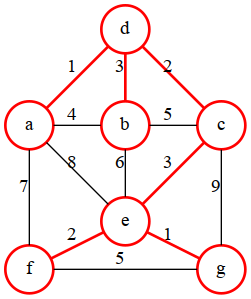
\includegraphics[width=0.33\textwidth]{graphs/minimum-spanning-trees/e_1_b_2.png}}~
 \subfloat[]{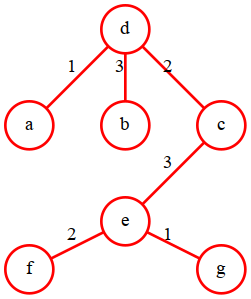
\includegraphics[width=0.33\textwidth]{graphs/minimum-spanning-trees/e_1_b_3.png}}
\end{figure}
\subsection{Shortest Paths}
\subsubsection{Dijkstra's Algorithm}
\subsubsection{A* Search}
\subsubsection{Bellman-Ford Algorithm}
\subsubsection{Floyd–Warshall Algorithm}
\end{document}
